\section{\StructurePackingSectionName}

\RU{Достаточно немаловажный момент, это упаковка полей в структурах\footnote{См. также: \URLWPDA}.}
\EN{One important thing is fields packing in structures\footnote{See also: \URLWPDA}.}

\RU{Возьмем простой пример:}\EN{Let's take a simple example:}

\lstinputlisting{patterns/15_structs/4_packing/packing.c}

\RU{Как видно, мы имеем два поля \Tchar (занимающий один байт) и еще два ~--- \Tint (по 4 байта).}
\EN{As we see, we have two \Tchar fields (each is exactly one byte) and two more~---\Tint (each - 4 bytes).}

\subsection{x86}

\RU{Компилируется это все в:}\EN{That's all compiling into:}

\lstinputlisting[caption=MSVC 2012 /GS- /Ob0,label=src:struct_packing_4,numbers=left]
{patterns/15_structs/4_packing/packing.asm.\LANG}

\RU{Кстати, мы передаем всю структуру, но в реальности, как видно, структура в начале копируется
во временную структуру (выделение места под нее в стеке происходит в строке 10,
а все 4 поля, по одному, копируются в строках 12 \ldots\ 19), 
затем передается только указатель на нее (или адрес).}
\EN{By the way, we pass a structure as a whole, but in fact, as we can see, the structure
is being copied to the temporary one (a place in stack is allocated in line 10 for it,
and then all 4 fields, one by one, is copied in lines 12 \ldots\ 19), 
then its pointer is to be passed (or address).}
\RU{Структура копируется, потому что неизвестно, будет ли ф-ция \TT{f()} модифицировать структуру.
И если да, то структура внутри \main должна остаться той же.}
\EN{The structure is copied, because it's unknown, will the f() function modify structure.
If it's so, then the structure inside of \main should remain as the same.}
\RU{Мы могли бы использовать указатели на \CCpp, и итоговый код был бы почти такой же,
только копирования не было бы.}
\EN{We could use pointers in \CCpp, and resulting code might be almost the same, but without
copying.}

\RU{Мы видим здесь что адрес каждого поля в структуре выравнивается по 4-байтной границе. 
Так что каждый \Tchar здесь занимает те же 4 байта что и \Tint. Зачем? 
Затем что процессору удобнее обращаться по таким адресам и кэшировать данные из памяти.}
\EN{As we can see, each field's address is aligned on a 4-bytes border.
That's why each \Tchar occupies 4 bytes here (like \Tint). Why?
Thus it is easier for CPU to access memory at aligned addresses and to cache data from it.}

\RU{Но это не экономично по размеру данных.}\EN{However, it is not very economical in size sense.}

\RU{Попробуем скомпилировать тот же исходник с опцией}\EN{Let's try to compile it with option} (\TT{/Zp1}) 
(\IT{/Zp[n] pack structures on n-byte boundary}).

\lstinputlisting[caption=MSVC 2012 /GS- /Zp1,label=src:struct_packing_1,numbers=left]
{patterns/15_structs/4_packing/packing_msvc_Zp1.asm.\LANG}

\RU{Теперь структура занимает 10 байт и все \Tchar занимают по байту. Что это дает? 
Экономию места. Недостаток ~--- процессор будет обращаться к этим полям не так эффективно 
по скорости, как мог бы.}
\EN{Now the structure takes only 10 bytes and each \Tchar value takes 1 byte. What it give to us?
Size economy. And as drawback~---CPU will access these fields without maximal performance it can.}

\label{short_struct_copying_using_MOV}
\RU{Структура так же копируется в \main. Но не по одному полю, а 10 байт, при помощи трех
пар \MOV.}
\EN{Structure is also copied in \main. Not by one-by-one field, but 10 bytes, using three pairs
of \MOV.}
\RU{Почему не 4?}\EN{Why not 4?}
\RU{Компилятор рассудил, что будет лучше скопировать 10 байт
при помощи 3 пар \MOV, чем копировать два 32-битных слова и два байта при помощи 4 пар \MOV.}
\EN{Compiler decided that it's better to copy 10 bytes using 3 \MOV pairs then to copy two 32-bit words
and two bytes using 4 \MOV pairs.}
\RU{Кстати, подобная реализация копирования при помощи \MOV взамен вызова ф-ции \TT{memcpy()}, например, это
очень распространенная практика, потому что это в любом случае работает быстрее чем вызов \TT{memcpy()} ---
если речь идет о коротких блоках, конечно: \ref{copying_short_blocks}.}
\EN{By the way, such copy implementation using \MOV instead of \TT{memcpy()} function calling is widely
used, because it's faster then to call \TT{memcpy()}---if to talk about short blocks, of course:
\ref{copying_short_blocks}.}

\RU{Как нетрудно догадаться, если структура используется много в каких исходниках и объектных файлах, 
все они должны быть откомпилированы с одним и тем же соглашением об упаковке структур.}
\EN{As it can be easily guessed, if the structure is used in many source and object files,
all these must be compiled with the same convention about structures packing.}

\newcommand{\FNURLMSDNZP}{\footnote{\href{http://msdn.microsoft.com/en-us/library/ms253935.aspx}
{MSDN: Working with Packing Structures}}}
\newcommand{\FNURLGCCPC}{\footnote{\href{http://gcc.gnu.org/onlinedocs/gcc/Structure_002dPacking-Pragmas.html}
{Structure-Packing Pragmas}}}

\RU{Помимо ключа MSVC \TT{/Zp}, указывающего, по какой границе упаковывать поля структур, есть также 
опция компилятора \TT{\#pragma pack}, её можно указывать прямо в исходнике. 
Это справедливо и для MSVC\FNURLMSDNZP и GCC\FNURLGCCPC{}.}
\EN{Aside from MSVC \TT{/Zp} option which set how to align each structure field, here is also
\TT{\#pragma pack} compiler option, it can be defined right in source code.
It is available in both MSVC\FNURLMSDNZP and GCC\FNURLGCCPC{}.}

\RU{Давайте теперь вернемся к \TT{SYSTEMTIME}, которая состоит из 16-битных полей. 
Откуда наш компилятор знает что их надо паковать по однобайтной границе?}
\EN{Let's back to the \TT{SYSTEMTIME} structure consisting in 16-bit fields.
How our compiler know to pack them on 1-byte alignment boundary?}

\RU{В файле \TT{WinNT.h} попадается такое:}\EN{\TT{WinNT.h} file has this:}

\begin{lstlisting}[caption=WinNT.h]
#include "pshpack1.h"
\end{lstlisting}

\RU{И такое:}\EN{And this:}

\begin{lstlisting}[caption=WinNT.h]
#include "pshpack4.h"                   // 4 byte packing is the default
\end{lstlisting}

\RU{Сам файл PshPack1.h выглядит так:}\EN{The file PshPack1.h looks like:}

\begin{lstlisting}[caption=PshPack1.h]
#if ! (defined(lint) || defined(RC_INVOKED))
#if ( _MSC_VER >= 800 && !defined(_M_I86)) || defined(_PUSHPOP_SUPPORTED)
#pragma warning(disable:4103)
#if !(defined( MIDL_PASS )) || defined( __midl )
#pragma pack(push,1)
#else
#pragma pack(1)
#endif
#else
#pragma pack(1)
#endif
#endif /* ! (defined(lint) || defined(RC_INVOKED)) */
\end{lstlisting}

\RU{Собственно, так и задается компилятору, как паковать объявленные после \TT{\#pragma pack} структуры.}
\EN{That's how compiler will pack structures defined after \TT{\#pragma pack}.}

\subsection{x86 + \olly + \RU{упаковка полей по умолчанию}\EN{fields are packed by default}}
\index{\olly}

\RU{Попробуем в \olly наш пример, где поля выровнены по умолчанию (4 байта)}
\EN{Let's try our example (where fields are aligned by default (4 bytes)) in \olly}: 
\figref{fig:packing_olly_4}.

\RU{В окне данных видим наши четыре поля}\EN{We see our 4 fields in data window}.
\RU{Вот только, откуда взялись случайные байты (0x30, 0x27) рядом с первым (a) и третьим (c) полем?}
\EN{But where from random bytes (0x30, 0x27) aside of first (a) and third (c) fields are came?}
\RU{Если вернетесь к листингу \ref{src:struct_packing_4}, то увидите, что первое и третье поле имеет
тип \Tchar, а следовательно, туда записывается только один байт, 1 и 3 соответственно (строки 6 и 8).}
\EN{By looking at our listing \ref{src:struct_packing_4}, we can see that first and third field
has \Tchar type, therefore, only one byte is written, 1 and 3 respectively (lines 6 and 8).}
\RU{Остальные три байта 32-битного слова не будут модифицироваться в памяти!}
\EN{Other 3 bytes of 32-bit words are not being modified in memory!}
\RU{А следовательно, там остается случайный мусор.}\EN{Hence, random garbage is there.}
\index{x86!\Instructions!MOVSX}
\RU{Этот мусор никак не будет влиять на работу \printf,
потому что значения для нее готовятся при помощи инструкции \MOVSX, которая загружает
из памяти байты а не слова}
\EN{This garbage influence \printf output in no way, because values for it is prepared
by \MOVSX instruction, which takes bytes, but not words}: 
\lstname \ref{src:struct_packing_4} (\RU{строки}\EN{lines} 34 \AndENRU 38).

\RU{Кстати, здесь используется именно \MOVSX (расширяющая знак), потому что тип \Tchar\EMDASH{}знаковый.}
\EN{By the way, \MOVSX (sign-extending) instruction is used here, because \Tchar type is signed.}
\RU{Если бы здесь был тип}\EN{If the type} \TT{unsigned char} \OrENRU \TT{uint8\_t}\EN{ be here}, 
\RU{то здесь была бы инструкция \MOVZX}\EN{\MOVZX instruction would be generated here instead}.

\begin{figure}[H]
\centering
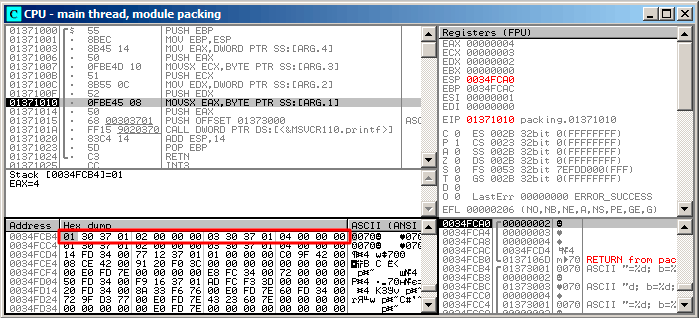
\includegraphics[scale=\FigScale]{patterns/15_structs/4_packing/olly_packing_4.png}
\caption{\olly: \RU{Перед исполнением \printf}\EN{Before \printf execution}}
\label{fig:packing_olly_4}
\end{figure}

\subsection{x86 + \olly + \RU{упаковка полей по границе в 1 байт}\EN{fields aligning by 1 byte boundary}}
\index{\olly}

\RU{Здесь всё куда понятнее: 4 поля занимают 10 байт и значения сложены в памяти друг к другу}
\EN{Things are much clearer here: 4 fields occupies 10 bytes and values are stored side-by-side}:
\figref{fig:packing_olly_1}.

\begin{figure}[H]
\centering
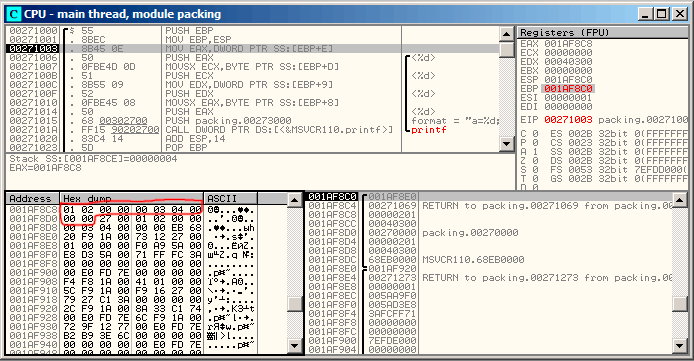
\includegraphics[scale=\FigScale]{patterns/15_structs/4_packing/olly_packing_1.png}
\caption{\olly: \RU{Перед исполнением \printf}\EN{Before \printf execution}}
\label{fig:packing_olly_1}
\end{figure}

\subsection{ARM + \OptimizingKeil + \ThumbMode}

\lstinputlisting[caption=\OptimizingKeil + \ThumbMode]{patterns/15_structs/4_packing/packing_Keil_thumb.asm}

\RU{Как мы помним, здесь передается не указатель на структуру, а сама структура, а так как в ARM первые 4 аргумента
функции передаются через регистры, то поля структуры передаются через}
\EN{As we may recall, here a structure passed instead of pointer to structure,
and since first 4 function arguments in ARM are passed via registers,
so then structure fields are passed via} \TT{R0-R3}.

\index{ARM!\Instructions!LDRB}
\index{x86!\Instructions!MOVSX}
\RU{Инструкция }\TT{LDRB} \RU{загружает один байт из памяти и расширяет до 32-бит учитывая знак.}
\EN{loads one byte from memory and extending it to 32-bit, taking into account its sign.}
\RU{Это то же что и инструкция}\EN{This is akin to} \MOVSX \RU{в}\EN{instruction in} x86.
\RU{Она здесь применяется для загрузки полей}\EN{Here it is used for loading fields} $a$ \AndENRU $c$ 
\RU{из структуры}\EN{from structure}.

\index{Function epilogue}
\RU{Еще что бросается в глаза, так это то что вместо эпилога функции, переход на эпилог другой функции!}
\EN{One more thing we spot easily, instead of function epilogue, here is jump to another function's epilogue!}
\RU{Действительно, то была совсем другая, не относящаяся к этой, функция, однако, она имела точно такой же
эпилог}\EN{Indeed, that was quite different function, not related in any way to our function, however, it has exactly
the same epilogue} 
(\RU{видимо, тоже хранила в стеке 5 локальных переменных}\EN{probably because, it hold 5 local variables too} 
($5*4=0x14$)).
\RU{К тому же, она находится рядом (обратите внимание на адреса).}
\EN{Also it is located nearly (take a look on addresses).}
\RU{Действительно, нет никакой разницы, какой эпилог исполнять, если он работает так же, как нам нужно.}
\EN{Indeed, there is no difference, which epilogue to execute,
if it works just as we need.}
\RU{Keil решил использовать часть другой ф-ции, вероятно, из-за экономии.}
\EN{Apparently, Keil decides to reuse a part of another function by a reason of economy.}
\RU{Эпилог занимает 4 байта, а переход ~--- только 2.}
\EN{Epilogue takes 4 bytes while jump~---only 2.}

\subsection{ARM + \OptimizingXcode + \ThumbTwoMode}

\lstinputlisting[caption=\OptimizingXcode + \ThumbTwoMode]{patterns/15_structs/4_packing/packing_Xcode_thumb.asm}

\index{ARM!\Instructions!SXTB}
\index{x86!\Instructions!MOVSX}
\TT{SXTB} (\IT{Signed Extend Byte}) \RU{это также аналог}\EN{is analogous to} \MOVSX \InENRU 
x86\RU{, только работает не с памятью, а с регистром.}\EN{ as well, but works not with memory, but with register.}
\RU{Всё остальное ~--- так же.}\EN{All the rest~---just the same.}

